\documentclass[11pt]{article}

\usepackage[margin=1in]{geometry}
\usepackage[T1]{fontenc}
\usepackage{lmodern}
\usepackage{microtype}
\usepackage{amsmath,amssymb,amsthm,mathtools}
\usepackage{mathrsfs}
\usepackage[dvipsnames]{xcolor}
\usepackage[most]{tcolorbox}
\usepackage{tikz}
\usetikzlibrary{decorations.markings,patterns}
\usepackage{enumitem}
\usepackage{tocloft}
\usepackage[hidelinks]{hyperref}

\definecolor{courseblue}{HTML}{1F4E79}
\definecolor{lightblue}{HTML}{EAF2F8}
\definecolor{lightgreen}{HTML}{EAF7EA}
\definecolor{lightpink}{HTML}{FCE8EF}
\definecolor{lightyellow}{HTML}{FFF8D6}
\definecolor{warningyellow}{HTML}{D6A000}
\definecolor{exercisebg}{HTML}{FDEAEA}
\definecolor{exerciseframe}{HTML}{B54040}
\definecolor{examplebg}{HTML}{F4FAFE}
\definecolor{exampleframe}{HTML}{85C1E9}
\definecolor{darkgray}{HTML}{333333}
\definecolor{lightorange}{HTML}{FDEBD8}
\definecolor{orangeframe}{HTML}{E08A3C}
\definecolor{remarkbg}{HTML}{F3EEFB}
\definecolor{remarkframe}{HTML}{9B7FC9}

\setlength{\parindent}{0pt}
\setlength{\parskip}{0.45em}
\setlist[itemize]{topsep=0.25em,itemsep=0.15em}
\renewcommand{\cftsecleader}{\cftdotfill{\cftdotsep}}
\renewcommand{\cftsubsecleader}{\cftdotfill{\cftdotsep}}

\theoremstyle{plain}
\newtheorem{theorem}{Theorem}[section]
\newtheorem{proposition}[theorem]{Proposition}
\newtheorem{lemma}[theorem]{Lemma}
\newtheorem{corollary}[theorem]{Corollary}
\theoremstyle{definition}
\newtheorem{definition}[theorem]{Definition}
\newtheorem{example}[theorem]{Example}
\newtheorem{exercise}[theorem]{Exercise}
\theoremstyle{remark}
\newtheorem*{remark}{Remark}
\newtheorem*{fact}{Fact}
\newtheorem*{warning}{Warning}

\tcolorboxenvironment{definition}{
  enhanced,
  unbreakable,
  colback=lightgreen,
  colframe=ForestGreen,
  boxrule=0.7pt,
  arc=2pt,
  left=6pt,
  right=6pt,
  top=5pt,
  bottom=5pt
}

\tcolorboxenvironment{remark}{
  enhanced,
  colback=remarkbg,
  colframe=remarkframe,
  before upper={\setlength{\parskip}{0.5em}},
  boxrule=0.7pt,
  arc=2pt,
  left=6pt,
  right=6pt,
  top=5pt,
  bottom=5pt
}

\tcolorboxenvironment{warning}{
  enhanced,
  colback=lightyellow,
  colframe=warningyellow,
  boxrule=0.7pt,
  arc=2pt,
  left=6pt,
  right=6pt,
  top=5pt,
  bottom=5pt
}

\tcolorboxenvironment{exercise}{
  enhanced,
  colback=exercisebg,
  colframe=exerciseframe,
  boxrule=1pt,
  arc=2pt,
  left=6pt,
  right=6pt,
  top=5pt,
  bottom=5pt
}

\tcolorboxenvironment{example}{
  enhanced,
  colback=examplebg,
  colframe=exampleframe,
  boxrule=0.7pt,
  arc=2pt,
  left=6pt,
  right=6pt,
  top=5pt,
  bottom=5pt
}

\numberwithin{equation}{section}

\newcommand{\be}{\begin{eqnarray}}
\newcommand{\ee}{\end{eqnarray}}
\newcommand{\C}{\mathbb{C}}
\newcommand{\R}{\mathbb{R}}
\newcommand{\N}{\mathbb{N}}
\newcommand{\Z}{\mathbb{Z}}
\DeclareMathOperator{\Log}{Log}
\DeclareMathOperator{\Arg}{Arg}

\DeclareMathOperator{\Hol}{\mathcal{H}\mathrm{ol}}
\DeclareMathOperator{\Real}{Re}
\DeclareMathOperator{\Imag}{Im}
\newcommand{\A}{\mathcal{A}}
\newcommand{\CT}{\C[[T]]}
\newcommand{\CLT}{\C((T))}
\tcbset{breakable}
% Compact spacing around diagrams; keep the main text at 11pt.
\newenvironment{lecturefigure}
 {\par\addvspace{0.25em}\begingroup\setlength{\parskip}{0pt}\centering}
 {\par\endgroup\addvspace{0.25em}}
\begin{document}

\begin{center}
  \colorbox{lightblue}{%
    \begin{minipage}{0.94\textwidth}
      \vspace{0.55em}
      \begin{tabular*}{\textwidth}{@{\extracolsep{\fill}}lr}
        {\color{courseblue}\bfseries\LARGE Lecture 20} &
        {\color{courseblue}\bfseries\LARGE MATH 411}\\[0.35em]
        \textbf{Fall 2026} & \textbf{Date: Oct 26, 2026}\\
        & \textbf{Instructor: Manish Patnaik}
      \end{tabular*}
      \vspace{0.45em}
    \end{minipage}}
\end{center}

\setcounter{tocdepth}{1}
\tableofcontents
\vspace{0.45em}

% Sources: the analyticity material removed from Lecture 19 (published
% version, Sections 4--5), handwritten Lecture 19, Oct. 26, pages 4--6,
% and handwritten Lecture 20, Oct. 28, pages 1--4 and the end of page 6.
% Order follows the handwritten Lecture 20: theorem, proof (kernel
% expansion, Cauchy formula, exchange of sum and integral, Cauchy
% estimates), derivatives, Liouville, and the fundamental theorem of
% algebra (handwritten Lecture 20, page 5). Morera's theorem and Laurent
% series (handwritten pages 6--9) are in Lecture 21.
In Lecture~19 we saw that every holomorphic branch of the logarithm is
given locally by a convergent power series. The logarithm illustrates a
general phenomenon: Cauchy's integral formula produces a convergent power
series for \emph{any} holomorphic function. We prove this, derive the
Cauchy estimates and Cauchy's formula for derivatives, and deduce
Liouville's theorem and the fundamental theorem of algebra.

\section{Holomorphic functions are analytic}
% Handwritten Lecture 19, page 4, and Lecture 20, page 1.
\begin{theorem}[Power series expansion and Cauchy estimates]\label{thm:analytic}
Let $U\subseteq\C$ be open and $f$ holomorphic on $U$. Suppose
$\overline{D(z_0,R)}\subseteq U$, where $R>0$, and let
$\gamma_R(t)=z_0+Re^{it}$, $0\leq t\leq2\pi$, be the positively
oriented boundary circle. Set
\[
 a_n:=\frac{1}{2\pi i}\int_{\gamma_R}
       \frac{f(\zeta)}{(\zeta-z_0)^{n+1}}\,d\zeta
 \quad(n\geq0),\qquad
 \|f\|_{\gamma_R}:=\max_{\zeta\in\gamma_R}|f(\zeta)|.
\]
Then
\begin{enumerate}
 \item $\displaystyle f(z)=\sum_{n=0}^{\infty}a_n(z-z_0)^n$
       for $|z-z_0|<R$;
 \item $\displaystyle |a_n|\leq\frac{\|f\|_{\gamma_R}}{R^n}$ for all $n\geq0$
       \quad\emph{(Cauchy estimates)}.
\end{enumerate}
The series converges uniformly on each closed disc
$\overline{D(z_0,s)}$ with $0<s<R$. Consequently, $f$ is analytic on $U$.
\end{theorem}

\begin{lecturefigure}
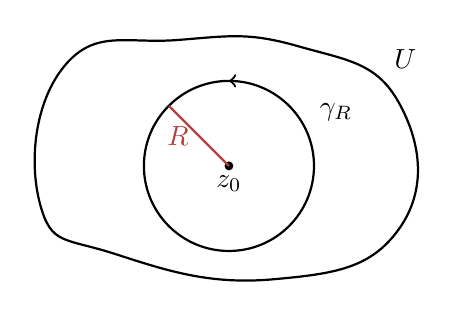
\begin{tikzpicture}[scale=0.8]
 \draw[thick] plot[smooth cycle,tension=0.8] coordinates
 {(-3,-0.6) (-2.6,1.6) (-0.8,2) (1.1,1.9) (2.7,1)
  (2.7,-1) (0.7,-1.8) (-1.8,-1.4)};
 \node at (2.8,1.7) {$U$};
 \draw[thick,postaction={decorate},decoration={markings,
 mark=at position 0.25 with {\arrow{>}}}] (1.35,0) arc(0:360:1.35);
 \fill (0,0) circle(2pt) node[below] {$z_0$};
 \draw[exerciseframe,thick] (0,0)--(-0.95,0.95) node[midway,left] {$R$};
 \node at (1.7,0.85) {$\gamma_R$};
\end{tikzpicture}
\end{lecturefigure}

\begin{remark}
\begin{itemize}
 \item The statement holds for \emph{every} closed disc
 $\overline{D(z_0,R)}\subseteq U$. The closed-disc condition ensures that
 $f$ is holomorphic on a neighborhood of the contour and its interior.
 \item In the formula for $a_n$, the integration variable $\zeta$ plays
 the role that $z$ played in Cauchy's formula; $z$ is reserved for the
 point where we evaluate $f$.
 \item For $n=0$, the coefficient formula is Cauchy's formula at the
 center: $a_0=f(z_0)$.
\end{itemize}
\end{remark}

\section{Proof of the power series expansion}
% Handwritten Lecture 19, pages 5--6, and Lecture 20, pages 1--4.
\subsection{Step 1: expand the Cauchy kernel}
For $\zeta\ne z$ and $\zeta\ne z_0$, write
\[
 \frac{1}{\zeta-z}
 =\frac{1}{(\zeta-z_0)-(z-z_0)}
 =\frac{1}{\zeta-z_0}\,\frac{1}{1-\dfrac{z-z_0}{\zeta-z_0}}.
\]
If $\bigl|\frac{z-z_0}{\zeta-z_0}\bigr|<1$, the geometric series gives
\begin{equation}\label{eq:kernel}
 \frac{1}{\zeta-z}
 =\frac{1}{\zeta-z_0}\left[1+\frac{z-z_0}{\zeta-z_0}
   +\left(\frac{z-z_0}{\zeta-z_0}\right)^2+\cdots\right]
 =\sum_{n=0}^{\infty}\frac{(z-z_0)^n}{(\zeta-z_0)^{n+1}}.
\end{equation}

To make the ratio uniformly small, fix $0<s<R$, so that
$D(z_0,s)\subseteq D(z_0,R)\subseteq U$. For $|z-z_0|\leq s$ and
$\zeta\in\gamma_R$ (so $|\zeta-z_0|=R$),
\[
 \left|\frac{z-z_0}{\zeta-z_0}\right|\leq\frac{s}{R}<1.
\]
Hence \eqref{eq:kernel} is valid for all such $z$ and $\zeta$, and the
$n$th term has absolute value at most $R^{-1}(s/R)^n$.

\begin{lecturefigure}
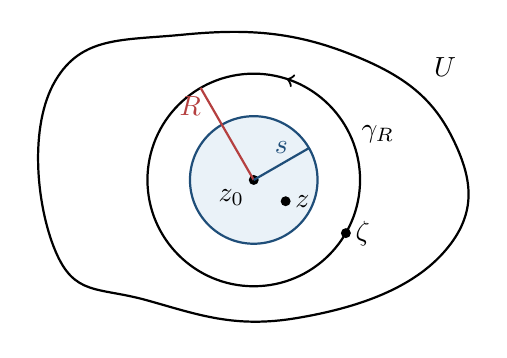
\begin{tikzpicture}[scale=0.9]
 \draw[thick] plot[smooth cycle,tension=0.75] coordinates
 {(-2.8,-1) (-2.8,1.4) (-1,2.05) (1.3,1.8) (2.8,0.6)
  (2.7,-1) (0.6,-1.95) (-1.5,-1.7)};
 \node at (2.7,1.6) {$U$};
 \draw[thick,postaction={decorate},decoration={markings,
 mark=at position 0.2 with {\arrow{>}}}] (1.5,0) arc(0:360:1.5);
 \draw[courseblue,thick,fill=lightblue] (0,0) circle(0.9);
 \fill (0,0) circle(2pt) node[below left] {$z_0$};
 \draw[exerciseframe,thick] (0,0)--(-0.75,1.3)
 node[pos=0.8,left] {$R$};
 \draw[courseblue,thick] (0,0)--(0.78,0.45) node[midway,above] {$s$};
 \fill (0.45,-0.3) circle(2pt) node[right] {$z$};
 \fill (1.3,-0.75) circle(2pt) node[right] {$\zeta$};
 \node at (1.75,0.65) {$\gamma_R$};
\end{tikzpicture}

{\small The smaller disc gives a uniform ratio $s/R<1$ on the contour.}
\end{lecturefigure}

\subsection{Step 2: apply Cauchy's integral formula}
Cauchy's integral formula (Lecture~18), applied to $|z-z_0|\leq s<R$
and the circle $\gamma_R$, gives
\[
 f(z)=\frac{1}{2\pi i}\int_{\gamma_R}\frac{f(\zeta)}{\zeta-z}\,d\zeta.
\]
Inserting the expansion \eqref{eq:kernel},
\[
 f(z)=\frac{1}{2\pi i}\int_{\gamma_R}
   \sum_{n=0}^{\infty}\frac{f(\zeta)}{(\zeta-z_0)^{n+1}}(z-z_0)^n\,d\zeta.
\]
\emph{If} we could exchange the sum and the integral, we would get
\[
 f(z)=\sum_{n=0}^{\infty}
 \underbrace{\left(\frac{1}{2\pi i}\int_{\gamma_R}
   \frac{f(\zeta)}{(\zeta-z_0)^{n+1}}\,d\zeta\right)}_{=\,a_n}(z-z_0)^n,
\]
which is the claimed expansion.

\subsection{Step 3: justify the exchange}
% Handwritten Lecture 20, page 3.
Recall that for a piecewise $C^1$ curve $\gamma$ and $g$ continuous on
$\gamma$, the ML estimate gives
\[
 \left|\int_\gamma g\right|\leq\operatorname{Length}(\gamma)\,\|g\|_\gamma.
\]

\begin{proposition}\label{prop:uniform-integral}
Let $\gamma$ be a piecewise $C^1$ curve, and let $(g_n)$ be a sequence of
continuous complex-valued functions on $\gamma$ converging uniformly on
$\gamma$ to a function $g$. Then
\[
 \lim_{n\to\infty}\int_\gamma g_n=\int_\gamma g.
\]
In particular, if each $h_k$ is continuous on $\gamma$ and the series
$\sum_{k=0}^{\infty}h_k$ converges uniformly on $\gamma$, then
\[
\int_\gamma\sum_{k=0}^{\infty}h_k=\sum_{k=0}^{\infty}\int_\gamma h_k.
\]
\end{proposition}
\begin{proof}
The limit $g$ is continuous, being a uniform limit of continuous
functions (Lecture~7), so $\int_\gamma g$ is defined. By the ML estimate,
\[
 \left|\int_\gamma g_n-\int_\gamma g\right|
 =\left|\int_\gamma (g_n-g)\right|
 \leq\operatorname{Length}(\gamma)\,\|g_n-g\|_\gamma
 \longrightarrow0,
\]
since $\|g_n-g\|_\gamma\to0$ by uniform convergence.

For the second statement, apply the first to the partial sums
$g_n=h_0+h_1+\cdots+h_n$ and use linearity of the integral.
\end{proof}

Now fix $z$ with $|z-z_0|\leq s$ and put
\[
 h_n(\zeta)=\frac{f(\zeta)(z-z_0)^n}{(\zeta-z_0)^{n+1}},\qquad\zeta\in\gamma_R.
\]
Each $h_n$ is continuous on $\gamma_R$ and
$|h_n(\zeta)|\leq\|f\|_{\gamma_R}R^{-1}(s/R)^n$. Hence the tail after
the $N$th term is bounded, uniformly in $\zeta\in\gamma_R$, by
\[
 \sum_{n=N+1}^{\infty}\frac{\|f\|_{\gamma_R}}{R}\Bigl(\frac sR\Bigr)^n
 =\frac{\|f\|_{\gamma_R}}{R}\,\frac{(s/R)^{N+1}}{1-s/R}\longrightarrow0.
\]
Thus the partial sums of $\sum h_n$ are uniformly Cauchy on $\gamma_R$,
so the series converges uniformly there (Lecture~7).
Proposition~\ref{prop:uniform-integral} justifies the exchange in Step~2,
giving $f(z)=\sum a_n(z-z_0)^n$ for $|z-z_0|\leq s$.

The tail bound is also independent of $z$ for $|z-z_0|\leq s$.
Integrating it over $\gamma_R$, whose length is $2\pi R$, gives
\[
 \sup_{|z-z_0|\leq s}
 \left|f(z)-\sum_{n=0}^{N}a_n(z-z_0)^n\right|
 \leq\|f\|_{\gamma_R}\,\frac{(s/R)^{N+1}}{1-s/R}\longrightarrow 0.
\]
Every point of $D(z_0,R)$ lies in such a disc, so the expansion holds throughout
$D(z_0,R)$. Finally, every $z_0\in U$ admits some $R>0$ with
$\overline{D(z_0,R)}\subseteq U$, so $f$ is analytic on $U$.

\subsection{Step 4: the Cauchy estimates}
% Handwritten Lecture 20, page 4.
On $\gamma_R$ we have $|\zeta-z_0|=R$, and $\operatorname{Length}(\gamma_R)=2\pi R$.
The ML estimate gives
\[
 |a_n|\leq\frac{1}{2\pi}\cdot\frac{\|f\|_{\gamma_R}}{R^{n+1}}
 \cdot2\pi R=\frac{\|f\|_{\gamma_R}}{R^n}.
\]
This completes the proof of Theorem~\ref{thm:analytic}. \hfill$\square$

\begin{remark}[Comparison with Hadamard's formula]
The Cauchy estimates give
$|a_n|^{1/n}\leq\|f\|_{\gamma_R}^{1/n}/R$, and
$\|f\|_{\gamma_R}^{1/n}\to1$ when $\|f\|_{\gamma_R}>0$
(if $\|f\|_{\gamma_R}=0$, all coefficients vanish). By Hadamard's formula
the radius of convergence $\rho$ of $\sum a_n(z-z_0)^n$ satisfies
\[
 \frac1\rho=\limsup_{n\to\infty}|a_n|^{1/n}\leq\frac1R,
 \qquad\text{that is,}\qquad \rho\geq R.
\]
So the Taylor series at $z_0$ converges on every disc centred at $z_0$
on which $f$ is holomorphic. For example, the Taylor series of an
\emph{entire} function at any point converges on all of $\C$.
\end{remark}

\section{Consequences}
\subsection{Derivatives and Cauchy's formula for derivatives}
% Handwritten Lecture 20, bottom of page 6.
A convergent power series $f(z)=\sum a_n(z-z_0)^n$ can be differentiated
termwise, and $a_n=f^{(n)}(z_0)/n!$. Comparing with
Theorem~\ref{thm:analytic}:

\begin{corollary}[Cauchy's integral formula for derivatives]\label{cor:derivatives}
If $f$ is holomorphic on $U$, then $f$ has derivatives of all orders on
$U$, each of which is holomorphic. If $\overline{D(z_0,R)}\subseteq U$, then
for every integer $n\geq0$,
\[
 \boxed{\displaystyle f^{(n)}(z_0)=\frac{n!}{2\pi i}\int_{\gamma_R}
 \frac{f(\zeta)}{(\zeta-z_0)^{n+1}}\,d\zeta,\qquad
 |f^{(n)}(z_0)|\leq\frac{n!\,\|f\|_{\gamma_R}}{R^n}.}
\]
\end{corollary}

\begin{remark}
We already knew that analytic functions are holomorphic by termwise
differentiation of power series. Theorem~\ref{thm:analytic} proves the
converse, so the two notions coincide. In particular, we may now replace
``analytic'' by ``holomorphic'' in the logarithm theorem of Lecture~19:
if $f$ is holomorphic and nonvanishing on a simply connected domain, then
$f'/f$ is holomorphic and $f$ has a holomorphic logarithm.
\end{remark}

\subsection{Liouville's theorem}
% Handwritten Lecture 19, pages 4--5, and Lecture 20, page 4.
\begin{corollary}[Liouville's theorem]\label{cor:liouville}
Every bounded entire function is constant.
\end{corollary}
\begin{proof}
Suppose $f$ is holomorphic on $\C$ and $|f(z)|\leq M$ for all $z$.
Expand at $z_0=0$. For every $R>0$, Theorem~\ref{thm:analytic} gives
\[
 f(z)=\sum_{n=0}^{\infty}a_n z^n\quad(|z|<R),\qquad
 |a_n|\leq\frac{\|f\|_{\gamma_R}}{R^n}\leq\frac{M}{R^n}.
\]
The coefficients are independent of $R$, since $a_n=f^{(n)}(0)/n!$.
For each fixed $n\geq1$, let $R\to\infty$; since $R^n\to\infty$, we get
$a_n=0$. Hence $f(z)=a_0$ on $D(0,R)$ for every $R$, i.e.\ on all of $\C$.
\end{proof}

\begin{lecturefigure}
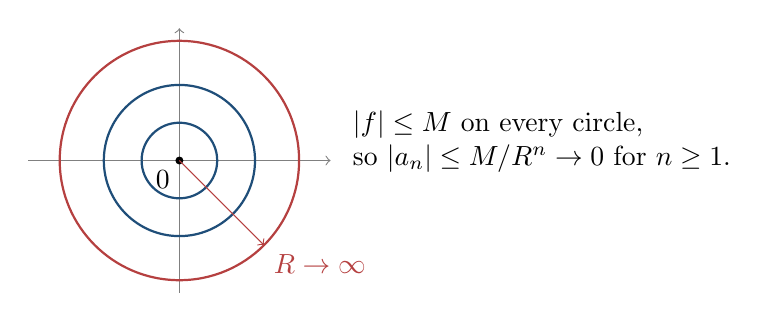
\begin{tikzpicture}[scale=0.8]
 \draw[gray,->] (-2.4,0)--(2.4,0);
 \draw[gray,->] (0,-2.1)--(0,2.1);
 \foreach \r/\c in {0.6/courseblue,1.2/courseblue,1.9/exerciseframe}
  \draw[\c,thick] (0,0) circle(\r);
 \fill (0,0) circle(1.8pt) node[below left]{$0$};
 \draw[exerciseframe,->] (0,0)--(1.343,-1.343) node[pos=1,below right]{$R\to\infty$};
 \node[right,align=left] at (2.6,0.3)
 {$|f|\leq M$ on every circle,\\so $|a_n|\leq M/R^n\to0$ for $n\geq1$.};
\end{tikzpicture}
\end{lecturefigure}

\begin{exercise}
Let $f$ be entire and suppose there are constants $C\geq0$ and $k\geq0$ with
$|f(z)|\leq C|z|^k$ for all $|z|\geq1$. Use the Cauchy estimates on
circles $|z|=R$ with $R\to\infty$ to show that $f$ is a polynomial of
degree at most $k$.
\end{exercise}

\subsection{The fundamental theorem of algebra}
% Handwritten Lecture 20, page 5.
\begin{theorem}[Fundamental theorem of algebra]\label{thm:fta}
Let $P(z)=a_nz^n+a_{n-1}z^{n-1}+\cdots+a_0$ be a polynomial with complex
coefficients, $n\geq1$ and $a_n\ne0$. Then $P$ has a root $\alpha\in\C$.
\end{theorem}
\begin{proof}
Suppose $P$ has no root. Then $1/P$ is entire. For $z\ne0$, factor out
the leading term:
\begin{equation}\label{eq:fta-factorization}
 P(z)=a_nz^n\left(1+\frac{b_1}{z}+\frac{b_2}{z^2}+\cdots+\frac{b_n}{z^n}\right),
 \qquad b_k=\frac{a_{n-k}}{a_n}.
\end{equation}
Put $B=|b_1|+\cdots+|b_n|$ and $\rho_0=\max(1,2B)$. For $|z|\geq\rho_0$,
\begin{equation}\label{eq:fta-tail-bound}
 \left|\frac{b_1}{z}+\cdots+\frac{b_n}{z^n}\right|
 \leq\frac{|b_1|+\cdots+|b_n|}{|z|}\leq\frac12.
\end{equation}
The first inequality uses the triangle inequality and $|z|\geq1$;
the second uses $|z|\geq2B$. By \eqref{eq:fta-factorization},
\eqref{eq:fta-tail-bound}, and the reverse triangle inequality,
\begin{equation}\label{eq:fta-polynomial-bound}
 |P(z)|\geq\frac{|a_n|}{2}|z|^n\geq\frac{|a_n|}{2},
\end{equation}
The first bound gives $|P(z)|\to\infty$ as $|z|\to\infty$; the second gives
$|1/P(z)|\leq2/|a_n|$ for $|z|\geq\rho_0$. On the compact disc
$|z|\leq\rho_0$, $1/P$ is continuous and hence bounded. Thus $1/P$ is
bounded and entire, so it is constant by Liouville's theorem. Then $P$
is constant, a contradiction.
\end{proof}

Next time we prove Morera's theorem and introduce Laurent series.

\end{document}
